%\pagestyle{fancy}
\chapter{Experimental Setup}
\label{ch:ExperimentalSetup}

\section{Sensors}
\subsection{\glsentrytext{imu}}
\missingfigure{Picture of myAHRS+ or/and ZED2i}
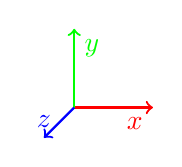
\begin{tikzpicture}
    \coordinate (O) at (0,0,0);
    \draw[thick,->, red] (0,0,0) -- (1,0,0) node[anchor=north east]{$x$};
    \draw[thick,->, green] (0,0,0) -- (0,1,0) node[anchor=north west]{$y$};
    \draw[thick,->, blue] (0,0,0) -- (0,0,1) node[anchor=south]{$z$};
\end{tikzpicture}
For the experiments the myAHRS+, a low cost high performance \acrfull{ahrs} will be used.
An \acrshort{ahrs} contains an \acrshort{imu} and outputs the raw data but also has an integrated Kalman filter which calculates the pose in form of quaternion or euler angles.
It offers an micro-USB interface and runs with up to \SI{100}{\Hz}.
It can capture a change of $\pm$2000 dps (degrees per second), $\pm$16 $g$ and $\pm$\SI{1200}{\micro\tesla}.
During the experiment only a fraction of this range is expected to be reached, hence the sensor seems suitable.
Besides the hardware the unit already has an Extended Kalman Filter (EKF) on board.
The EKF fuses the measurements of the three sensors and estimates a quaternion (and sth else?) from it.
But this will not be used.
\itodo{Also add ZED 2i \acrshort{imu} and compare (probably table similar to \acrshort{lidar})}


\subsection{\glsentrytext{lidar}}
Two different \acrshort{lidar}s will be used during the experiment.
The RS-Bpearl and the Velodyne UltraPuck.
The most relevant specifications of the two \acrshort{lidar}s can be seen in table \ref{tab:lidar_datasheets}.
Both are mechanical \acrshort{lidar}s and have the same number of laser channels, but the Velodyne has a significant better vertical resolution, due to the smaller vertical \acrshort{fov}.
\begin{table}[ht]
	\centering
	% todo: Manual citation prop wrong
	\caption{Comparison of the two used \acrshort{lidar}s \cite{RoboSense2020}\cite{Rev}}
	\label{tab:lidar_datasheets}
	\begin{tabular}[t]{lcc}
	\toprule
	&\textbf{RS-Bpearl} & \textbf{Velodyne Ultra Puck}\\
	\midrule
	Channels 					& 32 							& 32\\
	Range 						& \SI{100}{\metre}				& \SI{200}{\metre}\\
	Range accuracy				& $\pm\SI{3}{\centi\metre}$		& $\pm\SI{3}{\centi\metre}$\\
	Horizontal \acrshort{fov}	& \SI{360}{\degree}				& \SI{360}{\degree}\\
	Vertical \acrshort{fov} 	& \SI{90}{\degree} 				& \SI{40}{\degree} (\SIrange{-25}{15}{\degree})\\
	Horizontal resolution		& \SIrange{0.2}{0.4}{\degree} 	& \SIrange{0.1}{0.4}{\degree}\\
	Vertical resolution			& \SI{2.81}{\degree} 			& \SI{0.33}{\degree}\\
	Frame rate 					& \SIrange{10}{20}{\hertz}		& \SIrange{5}{20}{\hertz}\\
	Laser wavelength 			& \SI{905}{\nano\metre} 		& \SI{903}{\nano\metre}\\
	% \midrule
	Points per second 			& 576,000						& 600,000		\\
	\bottomrule
	\end{tabular}
	\end{table}%
\missingfigure{Picture of robosense or/and velodyne}



\section{Sensor placement}
\begin{figure}[htpb]
	\centering
	\documentclass{standalone}
\usepackage{tikz}
\usepackage{tikz-dimline}		% Dimension (measure) lines for TikZ
\usetikzlibrary{angles, calc, decorations.pathmorphing, quotes, spy}

\begin{document}
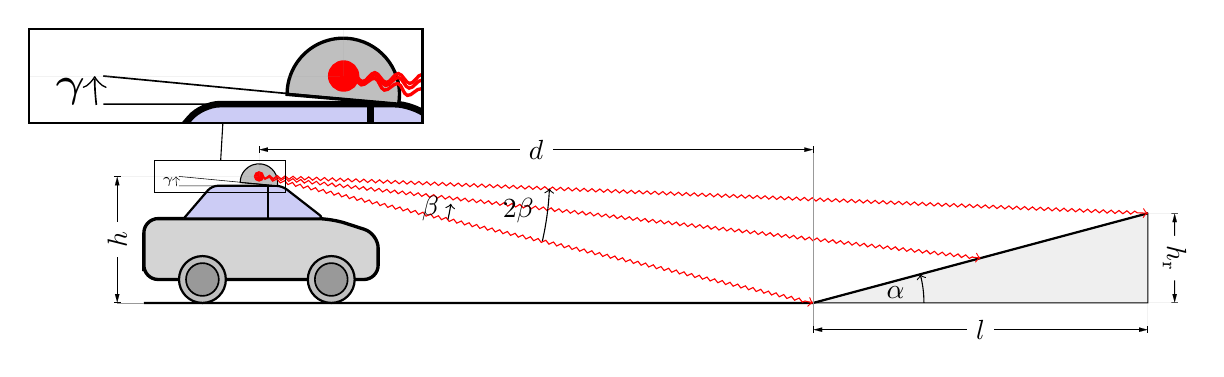
\begin{tikzpicture}[scale=0.85, spy using outlines={black, rectangle, magnification=3, width=5cm, height=1.2cm, connect spies}]
    % Define/Calc ramp parameters
    % Ramp length
    \def\rl{5};
    % Ramp angle [deg]
    \def\ra{15};
    % Ramp height
    \def\rh{{tan(\ra)*\rl}};
    % Distance of measurement line
    \def\dd{.4cm}

    % RAMP
    % Define the points
    \coordinate (A) at (0,0);
    \coordinate (B) at ($(A) + (\rl,0)$);
    \coordinate (C) at ($(B) + (0,\rh)$);
    % Draw and fill ramp
    \filldraw[draw=black, fill=lightgray!25] (A) -- (B) -- (C) -- cycle;
    % Draw angle
    \path (A) -- (B)
    pic[draw, ->, angle radius=40pt,
    angle eccentricity=0.75, "$\alpha$"]{angle=B--A--C};
    % Ground and helpers
    \coordinate (D) at ($(A) + (-10,0)$);
    \draw [thick] (D) -- (A) -- (C);

    % CAR
    \begin{scope}[scale=0.7]
        % Car height
        \def\ch{2}
        % Car length
        \def\cl{5}
        % Car body height
        \def\bh{\ch*0.65}
        % Roof length
        \def\rl{\cl*0.6}
        % Roof height
        \def\rh{\ch*0.35}
        % Car tilt angle
        \def\ct{6}
        % Anchor point is southwest
        \coordinate (b) at ($(D) + (0,0.5)$);
        % Offset to roof and wheels
        \coordinate (r) at ($(b) +(\cl*0.17,\ch*0.65)$);
        \coordinate (w) at ($(b) + (\cl*0.25,0)$);

        % Body
        \draw[black, fill=black!17, rounded corners=1.2ex, very thick]
        (b) -- ++(0,\bh) -- ++(\cl*1/5,0) --  ++(\cl*3/5,0) -- ++(\cl*1/5,-\bh*0.25)
        -- ++(0, -\bh*0.75) -- (b) -- cycle;
        % Roof
        \draw[very thick, rounded corners=0.5ex, fill=black!20!blue!20!white,thick]
        (r) -- ++(0.2*\rl,\rh) -- ++(0.5*\rl,0) -- ++(0.3*\rl,-\rh) -- (r);
        % \draw[thick] ($(r) + (\cl*0.5,\bh)$) -- ++(0,\rh);
        \draw[thick] (r)++(\rl*0.6,0) -- ++(0,\rh);

        % Wheels
        \draw[draw=black,fill=gray!50,thick] (w) circle (.5);
        \draw[draw=black,fill=gray!50,thick] (w) ++(\cl*0.55,0) circle (.5);
        % Inner wheels
        \draw[draw=black,fill=gray!80,semithick] (w) circle (.35);
        \draw[draw=black,fill=gray!80,semithick] (w) ++(\cl*0.55,0) circle (.35);

        % Lidar
        \draw[black, fill=gray!50] ($(r) + (\cl*0.40,\rh)$) coordinate (le) arc(-10:180:0.4) --cycle;

        % Car middle point
        \coordinate (m) at (\cl*0.5, \bh*0.5);
        % Lidar middle point
        \coordinate (lm) at ($(le) + (-0.39,0.2)$);
        \filldraw[red] (lm) circle(.1);
        % lidar mount angle
        % \draw (lm) -- ($(lm) + (-3, 0)$);
        % \path (A) -- (B)
        \coordinate (blob) at ($(le) + (-2.1, 0)$);
        \coordinate (blub) at ($(le) + (-2.1, 0.2)$);
        % \draw (blob) circle (.1);
        % \draw (blub) circle (.1);
        \draw[draw=black, very thin] (blob) -- (le) -- (blub)
        pic[draw, <-, angle radius=30pt,
        angle eccentricity=1.1, "\tiny $\gamma$"]{angle=blub--lm--blob};

        % Laser lines
        \draw[->,color=red,decorate,decoration={snake,amplitude=.2mm,segment length=1mm,post length=1mm}] (lm) -- (A);
        \draw[->,color=red,decorate,decoration={snake,amplitude=.2mm,segment length=1mm,post length=1mm}] (lm) -- ($(A)!0.5!(C)$);
        \draw[->,color=red,decorate,decoration={snake,amplitude=.2mm,segment length=1mm,post length=1mm}] (lm) -- ($(A)!1!(C)$);
        \path (lm) -- (A)
        pic[draw, ->, angle radius=70pt, angle eccentricity=0.9,
        "$\beta$"]{angle=A--lm--B};
        \path (lm) -- (C)
        pic[draw, ->, angle radius=105pt, angle eccentricity=0.9,
        "$2\beta$"]{angle=A--lm--C};
    \end{scope}

    % \dimline[extension start length=-\dd, extension end length=-\dd] {($(D)+(0,-\dd)$)}{($(A)+(0,-\dd)$)}{$d$};
    % \dimline[extension start length=\dd, extension end length=\dd] {($(A)+(0,-\dd)$)}{($(A)!0.4!(D)+(0,-\dd)$)}{$d$};
    \dimline[extension start length=\dd, extension end length=\dd+1.9cm] {($(lm)+(0,\dd)$)}{($(lm -| A)+(0,\dd)$)}{$d$};
    \dimline[extension start length=-\dd, extension end length=-\dd] {($(A)+(0,-\dd)$)}{($(B)+(0,-\dd)$)}{$l$};
    \dimline[extension start length=-\dd, extension end length=-\dd] {($(B)+(\dd,0)$)}{($(C)+(\dd,0)$)}{$h_\mathrm{r}$};
    \dimline[extension start length=\dd, extension end length=\dd+1.7cm] {($(D)+(-\dd,0)$)}{($(lm -| D)+(-\dd,0)$)}{$h$};
    % \draw (D) -- (lm -| D);
    % \dimline[extension start length=-\dd, extension end length=-\dd] {($(lm)+(\dd,0)$)}{($(C)+(\dd,0)$)}{$h_2$};
    % \dimline[extension start length=\dd, extension end length=\dd] {($(A)+(0,\dd)$)}{($(C)+(0,\dd)$)}{$d$};
    % \spy on ($(lm)!.05!(A)$) in node at (3,4);

    % \spy[black] on ($(lm) + (-0.42, 0)$) in node at (3,4);
    \spy on ($(lm) + (-0.5, 0)$) in node at ($(lm) + (-0.5, 1.5)$);

\end{tikzpicture}
\end{document}
	\caption{Mounting of the \acrshort{lidar}}
	\label{fig:tikz_lidar_mount}
\end{figure}
\itodo{\acrshort{imu} placement not really important, should just be static}
The \acrshort{lidar} will be placed on top of the car, to get a greater \acrshort{fov}.
The pitch angle at which the \acrshort{lidar} will be mounted should be chosen so that the number of points in the area at the beginning of the ramp are maximized.
This allows for an easier detection of planes with different inclination angles.
The coordinates at which the lasers hit the ground and ramp depend on the height of the \acrshort{lidar} $ h_\mathrm{L} $, the distance to the ramp $d$, the angle of the ramp $\alpha$, the pitch angle $\gamma$ at which the \acrshort{lidar} is mounted and finally on the vertical resolution and \acrshort{fov} of the \acrshort{lidar}. The coordinates can be calculated in the following way.\\
Assuming there is no ramp, the x-coordinate where the laser waves hit the ground can be calculated with
\begin{equation}
	x = \frac{h}{\tan(n\beta - \gamma)}
	\label{eq:ground_points}
\end{equation}
with $n$ being the "laserID" starting from the lowest opening angle and going to the highest.
When the ground is not a flat anymore, the assumption from \ref{eq:ground_points} does not hold anymore. The x distance between two laser points reduces on a ramp.
\dots whatever who cares
\itodo{Make a good sketch again with labels etc and check if its easy understandable, only then continue in tikz and latex}
\[ c = h - \frac{z}{\tan \alpha} \]
\itodo{\acrshort{lidar} pitch angle at which most point hit area before ramp can be calculated, explaination here using sketch \ref{fig:tikz_lidar_mount}}



\section{Car}
\missingfigure{Picture of eGolf}
\todoin{\begin{itemize}
	\item Some stats as height, track width etc, electric car hence less vibrations
	\item Problem with speed limit and odom (no odom when driving ramp up)
	\item Connection setup (maybe own section or maybe not interesting at all)
\end{itemize}
}



\section{Garage}
\missingfigure{Picture of ramps and/or figure of ramps showing angles}
\itodo{Think of a good way to measure the true angle of the ramps}